\documentclass[11pt]{extarticle}
\usepackage[utf8]{inputenc}
\usepackage{hyperref}
\usepackage{cite}
\usepackage[margin=1in]{geometry}
\usepackage{graphicx}
\usepackage{listings}
\usepackage{courier}
\usepackage{color}
\lstset{
    basicstyle=\footnotesize\ttfamily, % Default font
    % numbers=left,              % Location of line numbers
    numberstyle=\tiny,          % Style of line numbers
    % stepnumber=2,              % Margin between line numbers
    numbersep=5pt,              % Margin between line numbers and text
    tabsize=2,                  % Size of tabs
    extendedchars=true,
    breaklines=true,            % Lines will be wrapped
    keywordstyle=\color{red},
    frame=b,
    % keywordstyle=[1]\textbf,
    % keywordstyle=[2]\textbf,
    % keywordstyle=[3]\textbf,
    % keywordstyle=[4]\textbf,   \sqrt{\sqrt{}}
    stringstyle=\color{white}\ttfamily, % Color of strings
    showspaces=false,
    showtabs=false,
    xleftmargin=17pt,
    framexleftmargin=17pt,
    framexrightmargin=5pt,
    framexbottommargin=4pt,
    % backgroundcolor=\color{lightgray},
    showstringspaces=false
}
\usepackage{caption}
\DeclareCaptionFont{white}{\color{white}}
\DeclareCaptionFormat{listing}{\colorbox[cmyk]{0.43, 0.35, 0.35,0.01}{\parbox{\textwidth}{\hspace{15pt}#1#2#3}}}
\captionsetup[lstlisting]{format=listing,labelfont=white,textfont=white, singlelinecheck=false, margin=0pt, font={bf,footnotesize}}

%-------------------- Formatting

\setlength{\parindent}{2cm}
\setlength{\parskip}{8pt}

%-------------------- Title

\title{Concurrent SAT Solving with Identical Replicas}
\author{Julian Knodt, Sharad Malik}
\date{\today}
\begin{document}
\maketitle

%-------------------- Text

\section*{Introduction}
Existing SAT solvers mainly rely on single-threaded implementations, with most widely used SAT
solvers such as MiniSAT being single-threaded and not providing an alternate concurrent mode for
utilizing more resources for faster solving. There have been prior attempts to parallelize SAT
solvers, such as by partitioning the search space so that solvers can work on different
components without interfering with each other, or by creating a portfolio of solvers which have
been tuned to solve different problems more optimally. These approaches will sometimes share
information across solver instance, but since they often do not overlap in the search space,
they may not benefit from that sharing. If by keeping solvers searching similar portions we can
make sharing more efficient, we would like to see if maintaining multiple solvers with identical
hyper-parameters would lead still lead to a speed increase.
\section*{Overview}
While initially it seemed viable to build on top of minisat and demonstrate an increase in
speed, it was chosen instead to develop a new solver that would more adequately allow for the
inclusion of shared memory amongst solvers as MiniSAT relies heavily on being single-threaded in
order to allocate memory for clauses. Thus, it was decided to develop a new solver that might
better handle the concurrency constraints of the desired system. In addition, Rust was chosen as
the language of development due to how it handles safety with concurrent threads as well as its
efficiency. The solver to be developed was based heavily on MiniSAT\cite{minisat} with inspiration
from CryptoMiniSAT\cite{cryptoms} which has documented various aspects of implementing a SAT
Solver. In addition, various notes from Glucose\cite{glucose} and its parallel implementation were used.

The general steps of the algorithm are as follows:
\begin{lstlisting}[caption = Implementation Pseudocode]
// Parse clauses and literals from a dimacs file
fn parse_dimacs(filename) -> [Clauses];

// Create a Solver from a set of clauses;
fn make_solver([Clauses]) -> Solver;

// Takes one solver and creates multiple identical other solvers.
// These solvers all share the same database.
fn replicate(Solver, num_threads) -> [Solver];

// Solve clauses and return SAT w/ Solution or Unsat
fn solve(solver Solver) -> Option<Solution> {
  export_buffer: [Clause]
  import_buffer: [Clause]
  while solver.has_unassigned_variables() {
    solver.next_level()
    solver.choose_some_literal and assign()
    while solver.conflict() {
      if solver.level == 0 {
        return None
      }
      learnt, btlevel = solver.analyze(solver.conflict())
      solver.backtrack_to(btlevel)

      export_buffer.append(learnt)
      solver.add(asserting_literal(learnt))
      if not solver.conflict() {
        export(export_buffer)
        clear(export_buffer)
        import_from_others(import_buffer)
        while import_buffer.not_empty() {
          solver.add_imported(import_buffer.pop())
        }
      }
    }
    // no more conflicts
    solver.possibly_restart()
    solver.clean_old()
  }
  return Some(solver.current_assignment)
}

fn main(dimacs_filename, num_threads = 4) -> Nothing {
  clauses = from_dimacs(dimacs_filename)
  solver = make_solver(clauses)
  solvers = replicate(solver, num_threads)
  for solver in solvers {
    solve(solver)
  }
  solution = wait_any_solved(solvers)
  print(solution)
}
\end{lstlisting}

\section*{Project Tasks}
\begin{enumerate}
\item
In order to develop a multi-threaded SAT solver, it was necessary to create a single-threaded
SAT solver. Since MiniSAT is prominent and efficient, the overall algorithm, such as using
VSIDS, watch-lists, as well tracking various other metrics closely followed MiniSAT's
implementation. MiniSAT also has a custom arena based allocation for clauses, but this was not
implemented because it was unclear how this could be easily translated to a thread-safe
implementation. In addition, MiniSAT hand-rolled many different data-structures such as vectors,
maps, etc, but standard library versions were used in the new implementation, speeding up
development but possibly slowing down the final implementation. Of note, the standard library
version of HashMaps do not guarantee iteration order, so while the MiniSAT version is
deterministic in what order it traverses clauses, this implementation is not.

Building and development were all done through standard rust tooling(Cargo, rustc) and the
source code is available at \url{https://github.com/JulianKnodt/small_sat}.

This SAT solver, and also the final iteration of it, were limited in scope that they
could not be constructed at runtime, but instead just read in data from a CNF file\cite{cnf}.
This limitation did not matter, as it was the case that suitable CNF benchmarks exist and could
be used instead of hand-rolling benchmarks.

This implementation also changed the mutability of clauses, making it so that by defaults
clauses are sorted by the order of the literals, and that they are immutable. This was done to
make clauses more easily shared across threads, as in MiniSAT solvers would track which literal
was being watched by moving them to the front of the clause, but with multiple solvers tracking
literals, more than two literals might be tracked at the same time, so it would be impossible to
use that scheme in order to know which literals to look at. Thus, we explicitly track the other
literal in the clause being watched inside of the watch list itself.

\item
After implementing the initial version of the solver, it was necessary to add parallelization to
the solver. This was done by modifying the clause database to track clauses for $n$ different
solvers independently of each other, and also keeping a clock of the latest clause seen by each
solver. The clock was added in order to allow for garbage collection of clauses seen by all
solvers and also ensuring solvers were not being sent the same clause multiple times. It was
also necessary to use atomically reference counted pointers in order to share clauses across
threads, since we decided to use a shared memory model instead of allowing each thread to
allocate its own set of clauses. This, in hindsight, may have been a mistake as it became much
harder to handle garbage collection and ensuring only important clauses were kept in the solver,
as well as tracking clause activity.

Solvers could also share a solution with other solvers once it had found it, allowing for all
solvers to terminate once any one of them had either found a solution or found it unsatisfiable.

In addition, it was also thought that pinning each solver to a core might increase its
efficiency, as it would be able to best utilize its caches and the system as a whole.
Fortunately, there was an existing package \texttt{core\_affinity} which allowed for this. This
suggests to the system which core each thread should run on, and thus we run at most as many
threads as there are cores in order to hopefully gain the most benefit. On top of core affinity,
core exclusivity, where a thread is the only thing running on a core, was considered, but I am
unfamiliar with any tools that allow for this to occur.

\item
In order to test my implementation, we created multiple small sample CNF files in order to test
that our output would properly return SAT or UNSAT as well as handle edge cases such as
duplicate initial clauses and empty initial clauses properly. Then, various different
benchmarks were pulled from \url{https://www.cs.ubc.ca/~hoos/SATLIB/benchm.html}, and ran the
solver on them in order to test runtime performance. Specifically, iterating on the "Flat"
graph colouring instances and uniform random 3-SAT for a good portion of the single threaded
solver, and moving on to the SAT-encoded bounded model checking instances for longer runtimes
which more thoroughly test the solver. These timing tests were compared against the same solver
with a lower number of cores in order to analyze the results. These timing tests were run on an
a 4-core linux cluster which appeared to be mainly unused during the times tests were run.
\end{enumerate}

There were also issues that cropped up during development, and some of them are listed below:
\begin{enumerate}
\item
Conflict Clause simplification in MiniSAT has three levels, "deep", "basic", and "none". None is
where there is no minimization done, and the clause is not processed at all before being
returned, Basic is when literals are checked only one level deep if they are required or not,
which is done by checking if they are assigned at level 0, or they were between the UIP and the
conflict. Deep does this recursively, checking causes of each literal, and ensuring that all of
the parents are safe in order to more aggressively remove literals. Deep conflict clause
minimization in minisat is implemented as a stack based algorithm, performing depth first
search, checking parents before completing any one clause. I had initially implemented it as
breadth first, checking the entire clause, then checking parents. While this may seem like an
easily noticable bug, it was not evident for a good amount of time primarily because many
instances still appeared to be correctly solved, and it only sporadically returned an incorrect
answer. This made it appear as though for the most part minimization seemed to have work, and
the sporadic bug could've arisen from anywhere in the code. In addition, it dramatically
increased the speed of the solver in most cases, but also slowed things down without bounds in
other cases. This could possibly be due to creation of cycles, but it's unclear where they
could've been introduced. These speedups do give hope that there could be further advancement on
conflict clause minimization while still retaining correctness. Rather than explore fast
minimization though, I ended up reimplementing it as a recursive function for simplicity
reasons, despite the possibility of blowing up the stack.
\item
In order to rapidly develop the solver, multiple shortcuts were taken in its development in
order to more quickly build it at the cost of slower run times. Two key ones that were later
removed for optimization purposes were the inclusion of intermediate data structures and the
hashing and hashmap algorithm used in the solver.

Intermediate buffers between function calls allows for
easily returning data from any call and not immediately processing it, as it might be unclear
where it should be processed and how it should be processed. When it is more clear how the
results should be processed, these intermediate data structures are less efficient as they
require memory to be allocated. Thus, removing them lead to a decent speed increase.

The other key optimization was changing the hashing algorithm and hashmap type, as at the time
the builtin hashmap used a SipHash, designed to be strong against directed attempts at key
collision and fast for medium sized keys. Neither of these properties were desirable, as in this
implementation integer keys were used, and the hashmaps were all internal to the system.
Changing these properties significantly sped up the watch-list, and likely suggest I should
adopt MiniSAT's \texttt{IntMap} data structure as opposed to the builtin \texttt{HashMaps}.
\item
Another difficult to handle case was the representation of the \texttt{Clause} in memory. In
MiniSAT, it is represented as a header with information about the clause and a pointer into a
contiguous array of literals. I originally went with the simplification that clauses own the
literals which they contain as this would more easily allow clauses to be shared across
different threads. Since shared memory was used, such a scheme seemed necessary, but it is
likely possible to structure the system to both efficiently use arena allocation of literals
and provide thread-safety for shared clauses.
\end{enumerate}
\section*{Results}
% Details of experimentation result & implementation status
% TODO add plots here
Currently, the solver works correctly and fairly efficiently. It currently allows for multiple
threads to be run, and running multiple threads shows an increase in speed when adding more
cores, as shown by the graphs below over a given set of benchmarks, as was desired, but not
quite as much as was hoped for. Initially, we considered that it might be the case that if the
solvers could stay almost in lock-step, they might be able to gain a superlinear speedup due to
the ability for solvers to send relevant clauses when other solvers might need them. That does
not appear to be the case though, as at best it appears to be a linear speedup. Hopefully these
speed-ups would apply in the case of a further optimized solver, and more work must be done in
order to verify that that is the case.

Below are the timing results from running the solver over the collection of bounded model
checking benchmarks. They were run on a Linux Cluster with no other workload during the running
time, and 100 sample points for each file were collected, and each thread for each solver
reported its running time. Thus, for four cores, it reported 400 data points per file, 300 for
three cores, and so forth. We expect each of the samples to be identically distributed and
independent from other samples.


\noindent
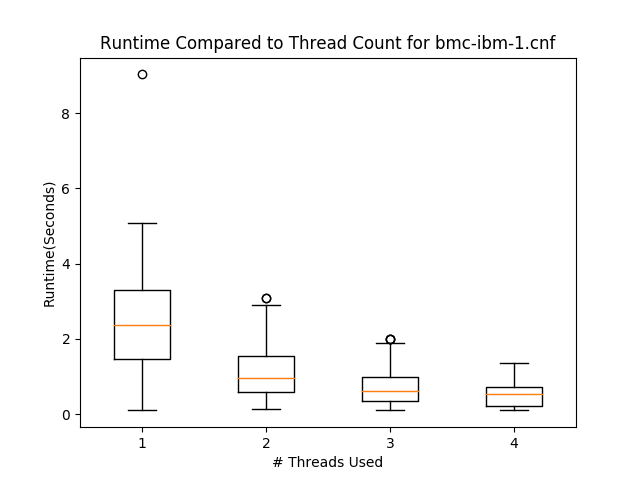
\includegraphics[width=0.5\textwidth]{figures/bmc-ibm-1.png}
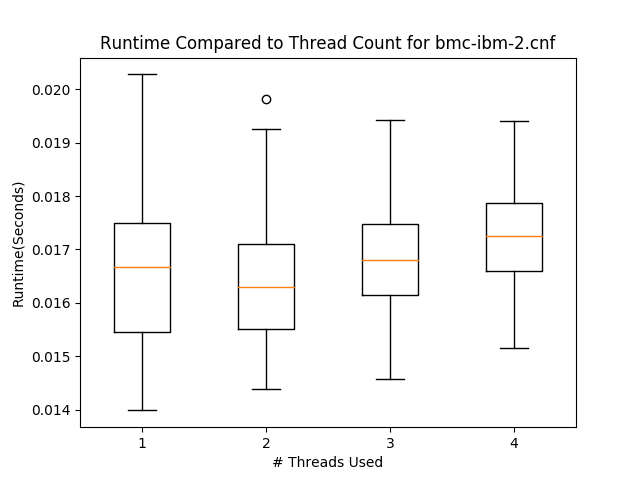
\includegraphics[width=0.5\textwidth]{figures/bmc-ibm-2.png}
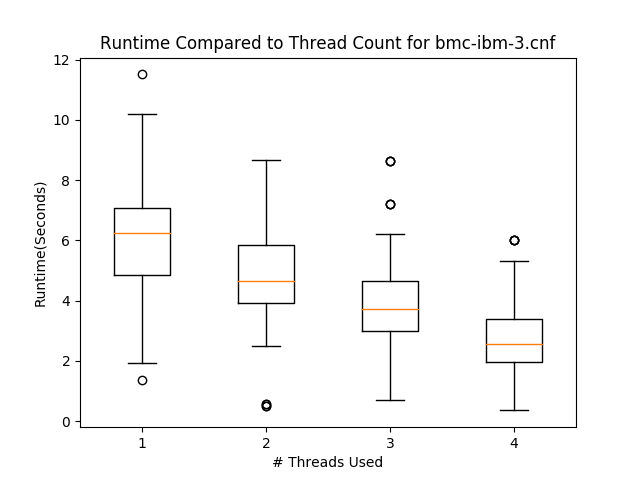
\includegraphics[width=0.5\textwidth]{figures/bmc-ibm-3.png}
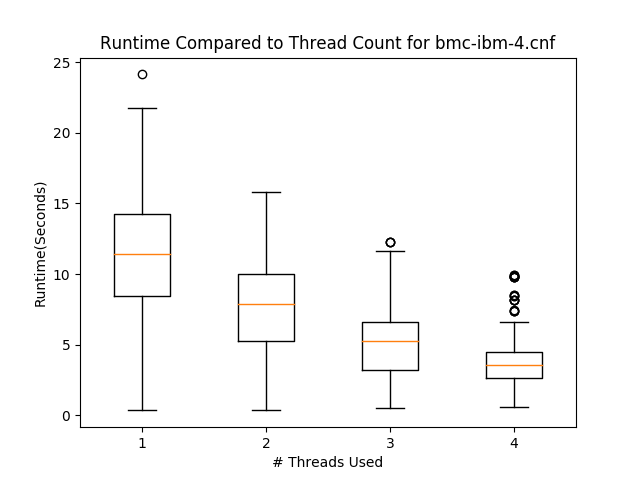
\includegraphics[width=0.5\textwidth]{figures/bmc-ibm-4.png}
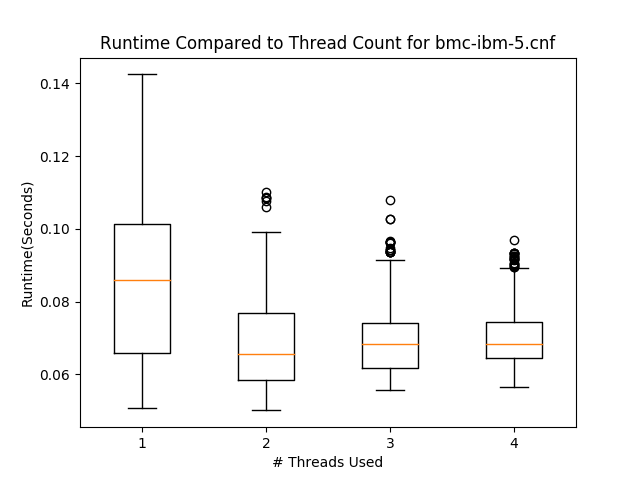
\includegraphics[width=0.5\textwidth]{figures/bmc-ibm-5.png}
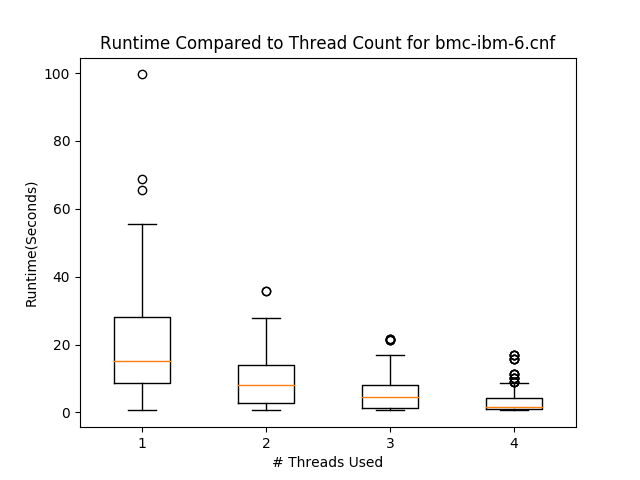
\includegraphics[width=0.5\textwidth]{figures/bmc-ibm-6.png}
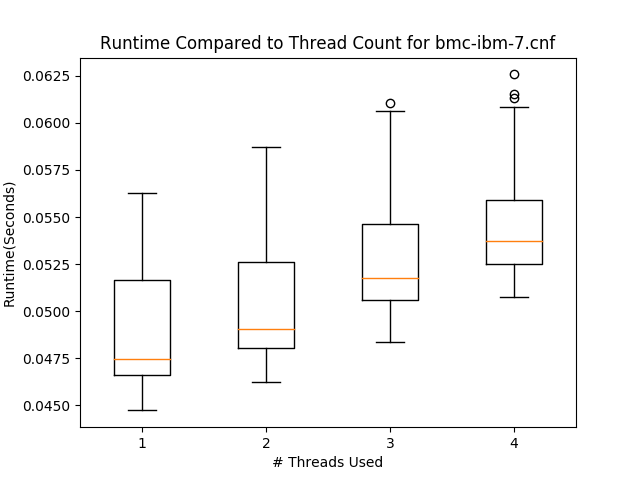
\includegraphics[width=0.5\textwidth]{figures/bmc-ibm-7.png}
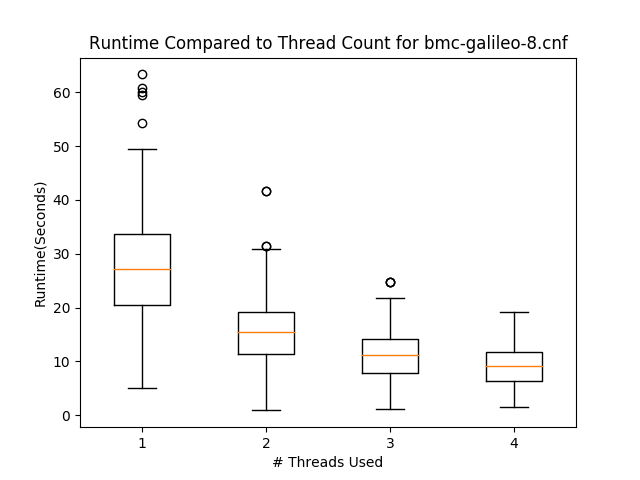
\includegraphics[width=0.5\textwidth]{figures/bmc-galileo-8.png}
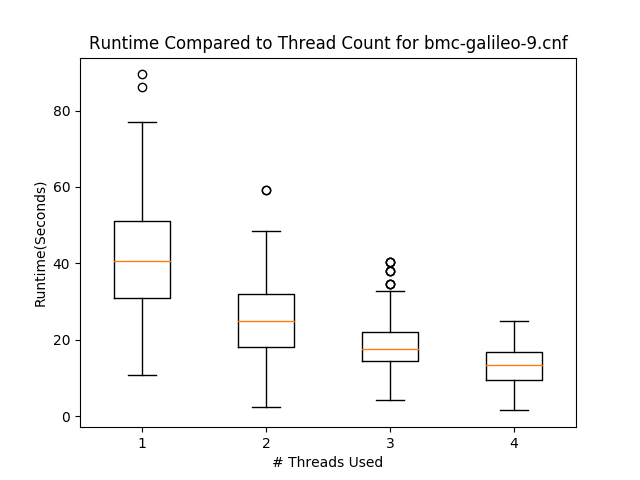
\includegraphics[width=0.5\textwidth]{figures/bmc-galileo-9.png}
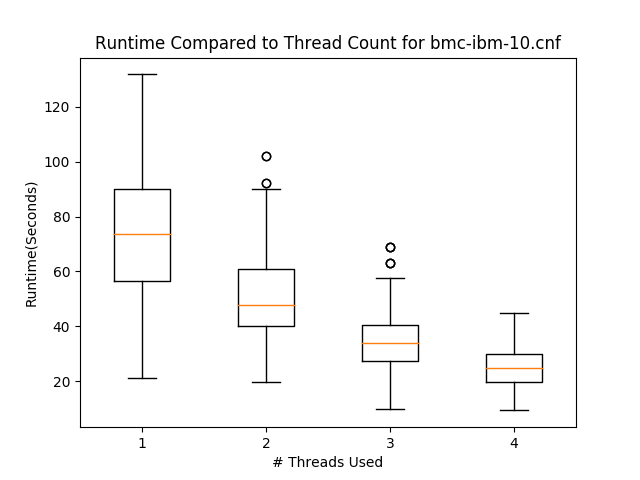
\includegraphics[width=0.5\textwidth]{figures/bmc-ibm-10.png}
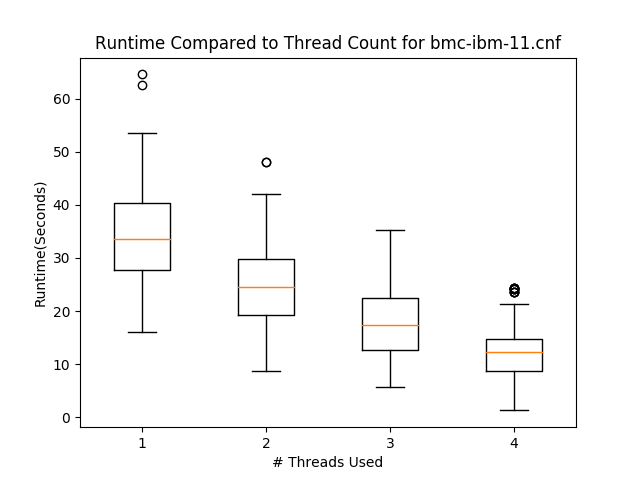
\includegraphics[width=0.5\textwidth]{figures/bmc-ibm-11.png}
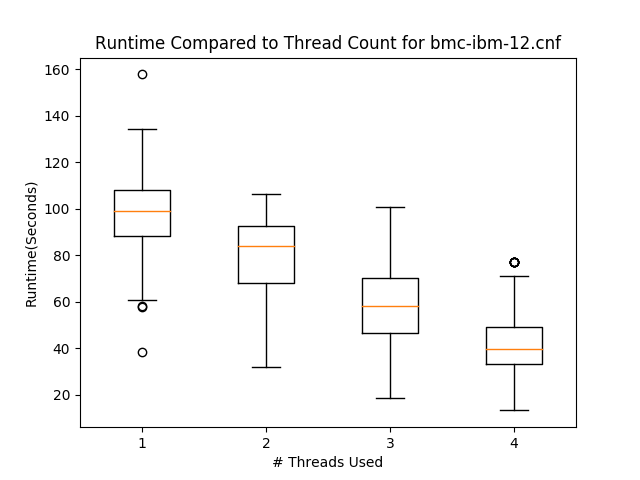
\includegraphics[width=0.5\textwidth]{figures/bmc-ibm-12.png}
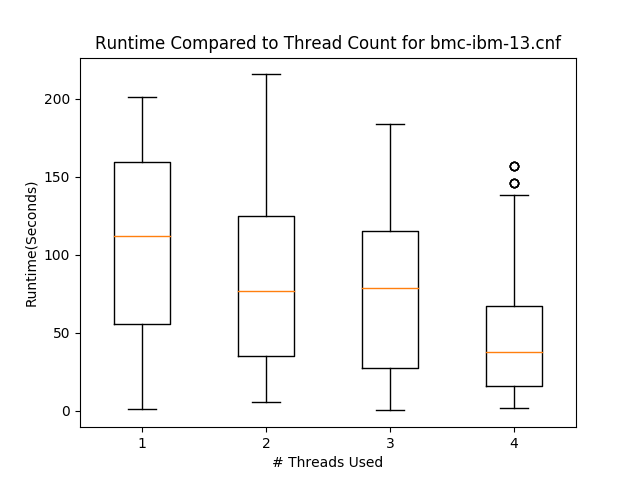
\includegraphics[width=0.5\textwidth]{figures/bmc-ibm-13.png}


By looking at the samples taken, we can see there is a clear linear trend in the runtime per
thread. In some cases though, as in \texttt{bmc-ibm-11}, it appears that adding more cores
becomes less effective the more cores are added. This might be the case because each thread
might diverge more from other threads on longer instances. In addition, for the case of the
\texttt{bmc-ibm-*.cnf} files, it is the case that many clauses are binary, so some learnt clauses
and implications for the solvers will be the same, thus it is expected that some of the shared
work is not necessary.

It should also be noted that the variance in most cases tends to decrease the more cores there
are. This intuitively makes sense, as if one core gets stuck searching a part of the search
space with no solution, if there are other solvers exploring more useful parts it is more likely
that it will find an answer quickly. In the cases where variance did not stay the same, we
suspect it to be the fault of the implementation, as it might be the case that allocations could
cause random pauses which cannot be accounted for.

There are also multiple cases where it appears that adding more cores is slower than using a
single core. These cases are where the time in order to create multiple solvers significantly
outweighs the benefit of having them, as these cases often have runtimes in the tens of
milliseconds. For these smaller instances, the necessity of copying separate watchlists for each
of the threads is likely the cause of slowdown. Interestingly, it appears that despite the
slowdown of copying memory, two cores slightly outperformed one core, so it might still be
worthwhile to have multiple cores. It is also unclear whether from the initial set of clauses if
specific instances can be determined to better utilize more cores, and if so whether that
information can be used to more efficiently use resources.

\section*{Discussion}
% What worked, what didn't & why
Handling concurrency was the most successful portion of this project, as it was the case that
creating multiple instances of the same solver and sharing data between them was fairly easy to
implement and bug free. Core affinity was also easily added into the project. This is mainly due
to the strong type system provided by the tooling used, and also the ease of use of the package
manager which allowed for quick integration of existing work. Unlike MiniSAT, the compilation
process was also extremely simple, as the language and compiler properly handle compiling for
different architectures and libraries don't need to be manually linked. Thus, what might've been
a large hiccup in previous tooling was very smooth given the state of new tools. This allowed a
fairly efficient implementation of clause sharing which demonstrated the effectiveness of it.

On the other hand, the new system still does not have the ability to easily implement everything
that can be implemented in C++. For example, controlling arena allocation is not as easy, and
there are no pre-existing implementations which are well explained. In addition, while it is
much safer to implement concurrent programs, it also becomes much harder to correctly and
efficiently implement. This difficulty also comes from the type system, which enforces many
invariants which are hard to reason about. This ends up being a win for correct implementations
of algorithms, but forces more time spent on API design and ensuring these invariants are
satisfied.
\section*{Conclusions}
% Future directions & summary
We were able to implement a SAT solver which correctly solves instances at a respectable rate.
In addition, we demonstrated the effectiveness of running multiple solvers with the same
parameters and clause sharing, which seems to be generally a linear speed up compared to a
single threaded implementation. This shows that it might be useful to further explore more
effective ways of clause sharing and clause memory sharing.

In terms of future work, there are multiple different approaches which can be taken in order to
improve the efficiency of SAT solvers both in concurrent and single-threaded contexts.

\begin{enumerate}
\item
Developing a scheme that allows solvers to specify which clauses are relevant to them and only
retrieve clauses from other solvers which fit this criteria. Currently, a source of inefficiency
in the system is sending clauses which may never be used in unit propogation, which slows down
the efficiency of the watch-list as more clauses on average must be checked before any of them
allows for unit propogation. In this case, existing solvers take different approaches to this,
such as only watching one literal in transferred clauses, or only exporting clauses which only
fit certain criteria. In contrast, the solver itself is probably the most fit for knowing which
clauses might be relevant to it at the current moment. Creating some efficient way for each
solver to import relevant clauses using some metric, possibly such as VSIDS, might possibly
increase the efficiency of clause sharing. This might be an interesting avenue, as I'm not aware
of any existing systems which use this.
\item
Further optimizations to the current solver such as fixing memory accesses and the like would
probably be an interesting project. Unfortunately, optimizing to compete against a single-thread
solver with something that must properly handle multi-threading is much harder. To compete
against MiniSAT, a different approach would have to be taken in order to properly handle
optimizing for the single-threaded case so that stronger memory guarantees can be taken
advantage of, and also properly handle the multi-threaded case. In order to do so, it would
likely make sense to structure most of the codebase in a different way, likely suggesting a
rewrite of most of it. While this might be the most work intensive option, it is likely the most
effective for properly optimizing.

During the development of the solver, it became apparent that the efficiency of MiniSAT is due
to both the many optimizations made to the problem such as VSIDS, watch-lists, conflict clause
minimization, removal of already satisfied clauses, and the like, but also the high level of
care taken into ensuring that memory is used efficiently and that data structures are optimized
for their exact use case. This painstaking care is hard to match in a short amount of time, and
it requires a lot of prior experience to know exactly where to make each optimization.
\item
Instead of optimizing, there are also new features of SAT solvers, such as conversion to CNF
from other expressions, as well as the inclusion of other operators such as \texttt{XOR}. Adding
them to the solver would be an interesting way to understand what optimizations new solvers are
using.
\end{enumerate}

\section*{Appendix}
% Extra graphs
For completeness, other output stats from the solver are recorded here, as they can also be used
to measure performance of the solver. They are also indicative of the new features of the
solver, and help demonstrate the relation of threads to other components.

\subsubsection*{Clauses Imported from other Solvers}

In order to share clauses, solvers "import" clauses from other threads in bulk. These clauses
are then added to the watchlist one-by-one so that they can be used in unit propogation.
We simply recorded the bulk amount imported, in order to get a better understanding of how many
extra clauses each solver was getting.

\noindent
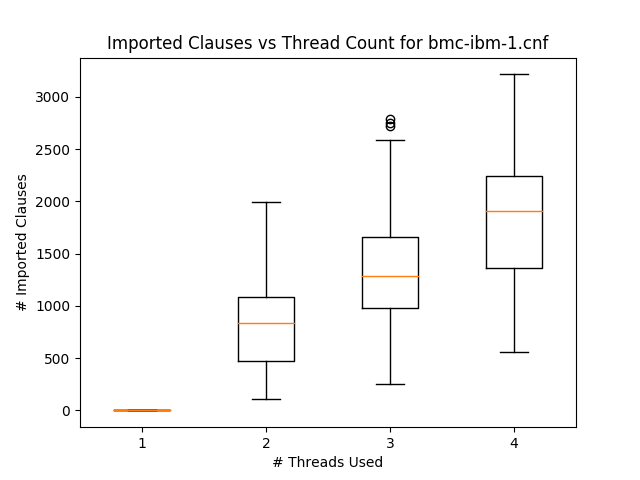
\includegraphics[width=0.25\textwidth]{figures/bmc-ibm-1imp.png}
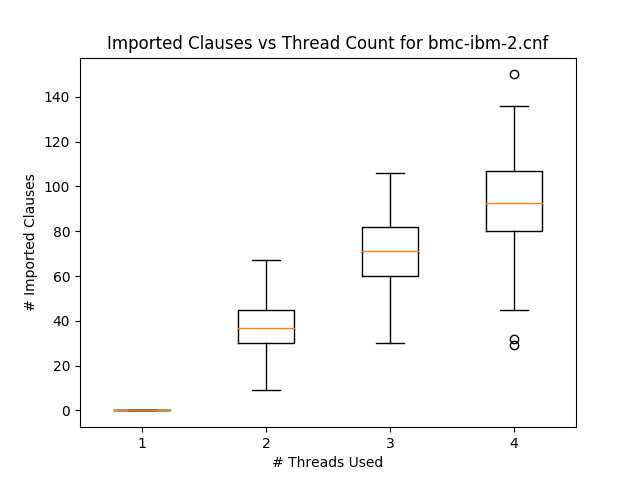
\includegraphics[width=0.25\textwidth]{figures/bmc-ibm-2imp.png}
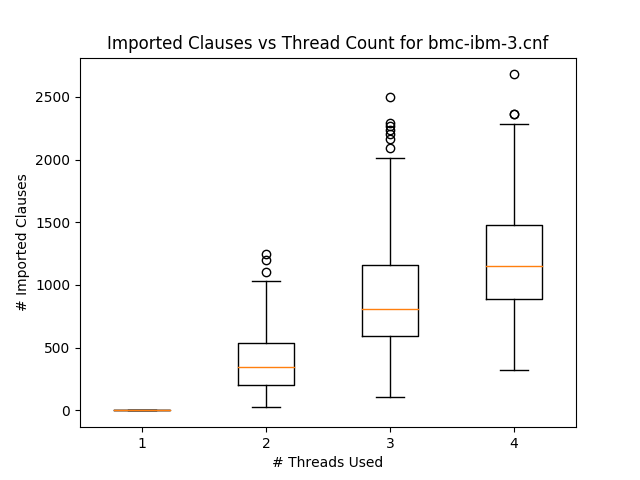
\includegraphics[width=0.25\textwidth]{figures/bmc-ibm-3imp.png}
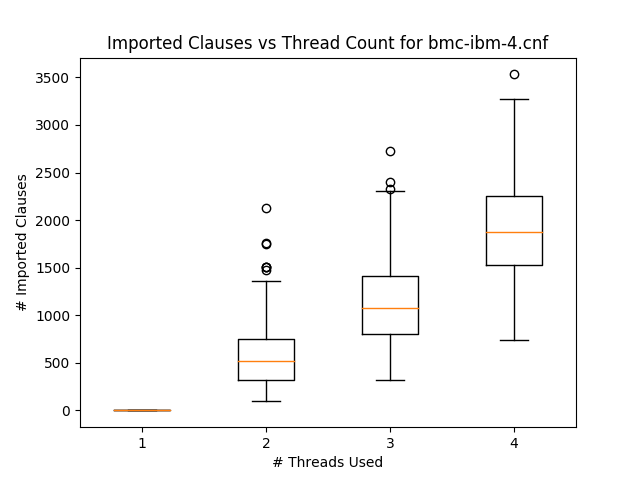
\includegraphics[width=0.25\textwidth]{figures/bmc-ibm-4imp.png}
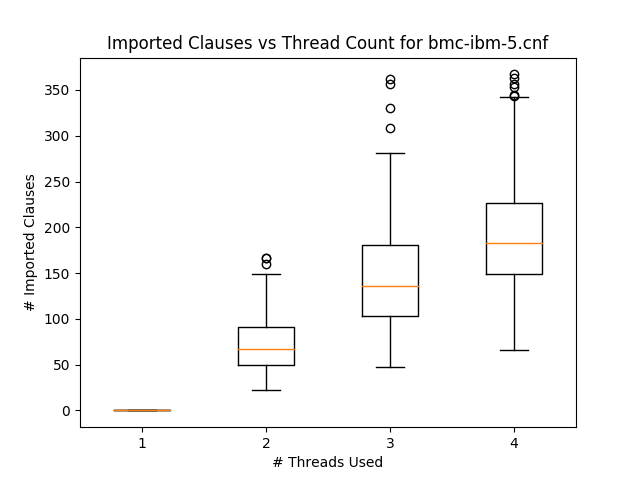
\includegraphics[width=0.25\textwidth]{figures/bmc-ibm-5imp.png}
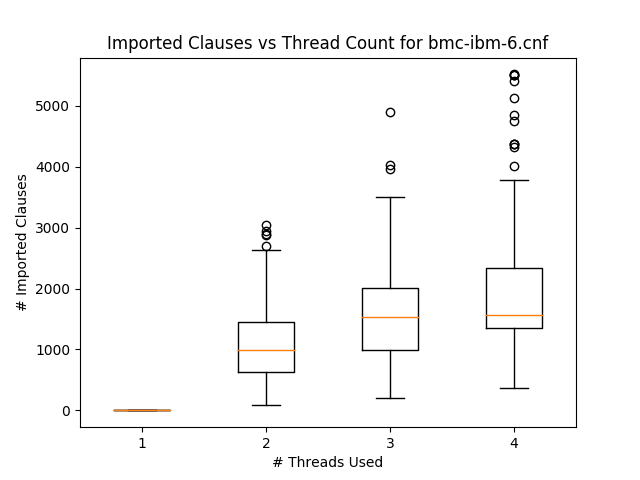
\includegraphics[width=0.25\textwidth]{figures/bmc-ibm-6imp.png}
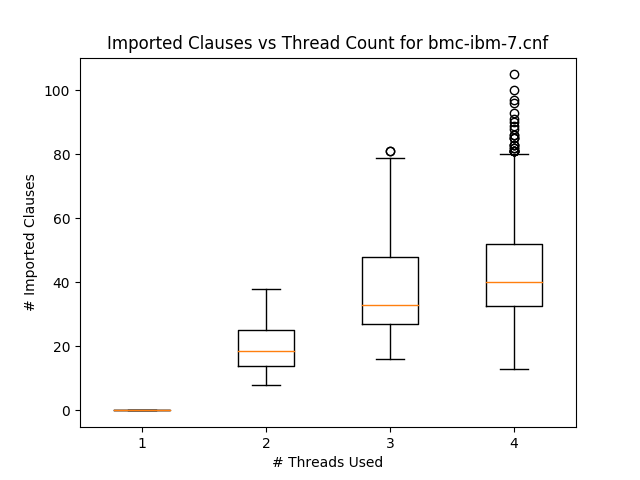
\includegraphics[width=0.25\textwidth]{figures/bmc-ibm-7imp.png}
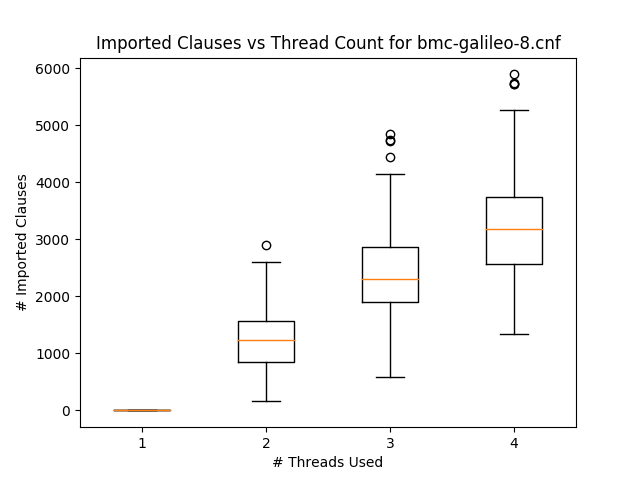
\includegraphics[width=0.25\textwidth]{figures/bmc-galileo-8imp.png}
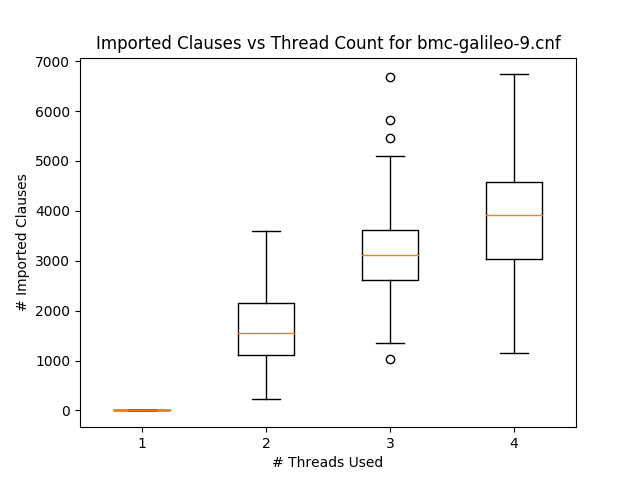
\includegraphics[width=0.25\textwidth]{figures/bmc-galileo-9imp.png}
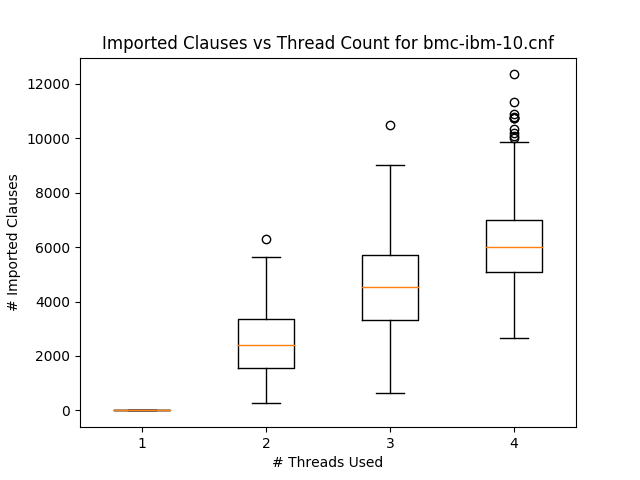
\includegraphics[width=0.25\textwidth]{figures/bmc-ibm-10imp.png}
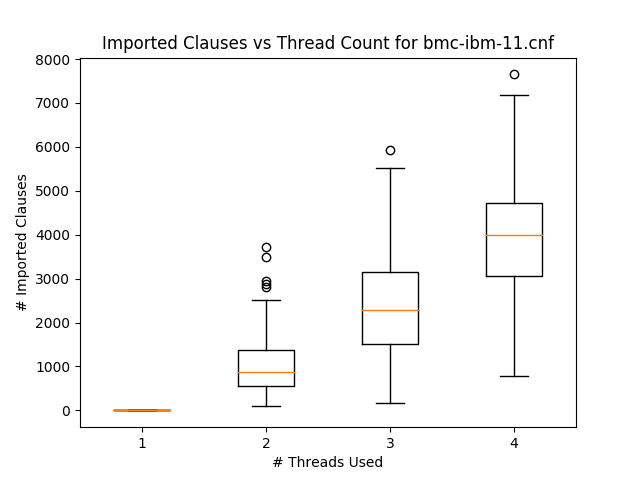
\includegraphics[width=0.25\textwidth]{figures/bmc-ibm-11imp.png}
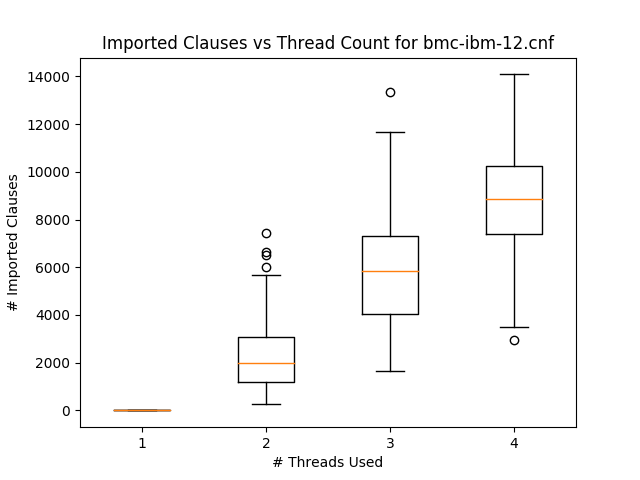
\includegraphics[width=0.25\textwidth]{figures/bmc-ibm-12imp.png}
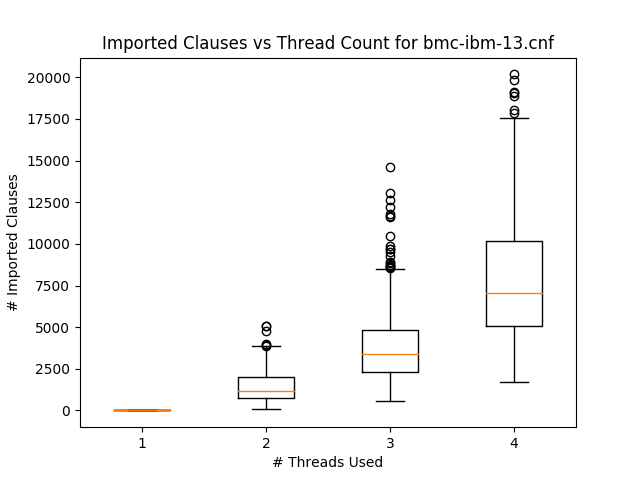
\includegraphics[width=0.25\textwidth]{figures/bmc-ibm-13imp.png}

It can be seen that as more threads are utilized, each individual thread gets significantly more
clauses imported with variance increasing significantly with more threads. Further analysis
would be required in order to determine what percentage of these imported threads are actually
used. It is also degenerate in the case of 1 thread, as there are no clauses to be imported.

\subsubsection*{Clauses Learned Per Thread}

This is one of the statistics used in MiniSAT, which is a record of how many clauses each thread
learns. That is, everytime it reaches a a conflict, it marks it as a time a clause was learnt.

\noindent
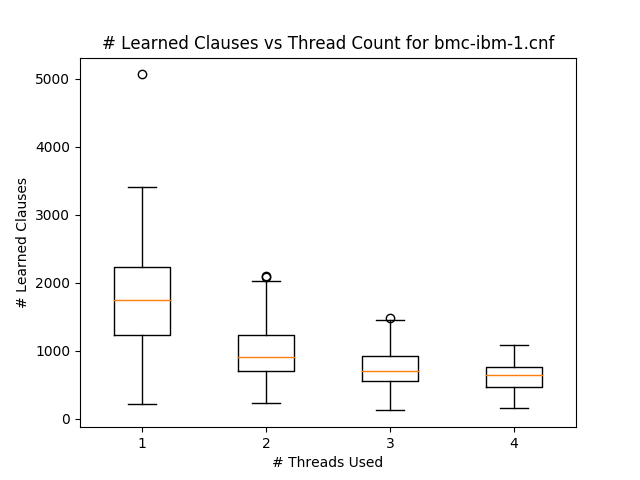
\includegraphics[width=0.25\textwidth]{figures/bmc-ibm-1lnt.png}
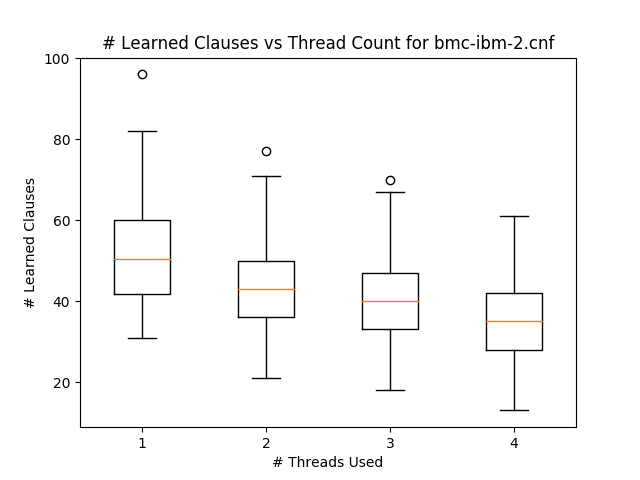
\includegraphics[width=0.25\textwidth]{figures/bmc-ibm-2lnt.png}
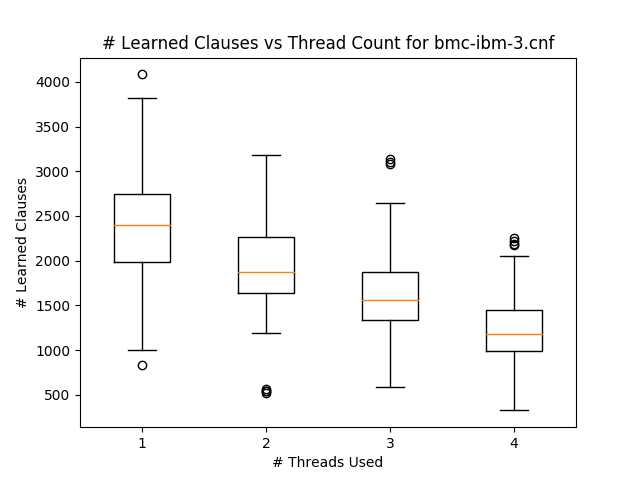
\includegraphics[width=0.25\textwidth]{figures/bmc-ibm-3lnt.png}
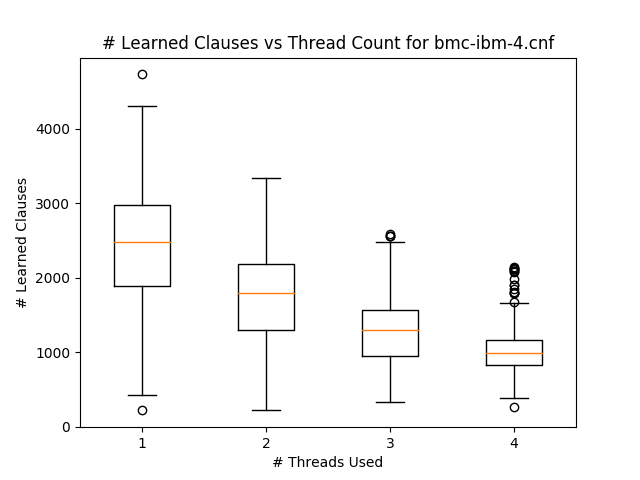
\includegraphics[width=0.25\textwidth]{figures/bmc-ibm-4lnt.png}
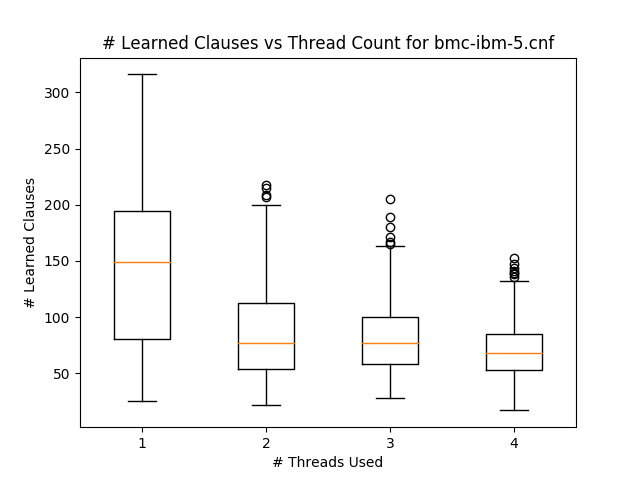
\includegraphics[width=0.25\textwidth]{figures/bmc-ibm-5lnt.png}
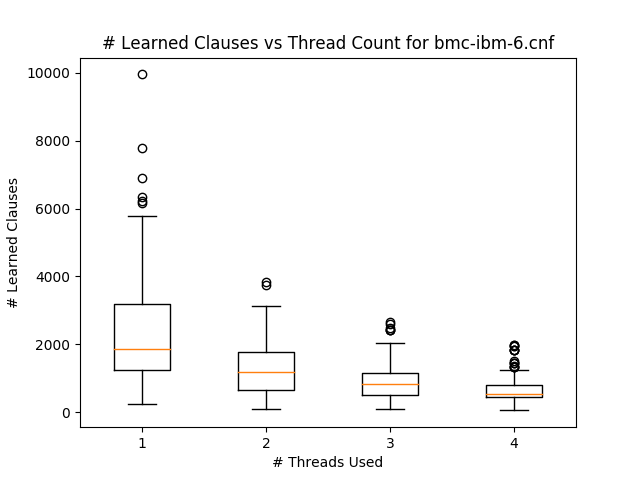
\includegraphics[width=0.25\textwidth]{figures/bmc-ibm-6lnt.png}
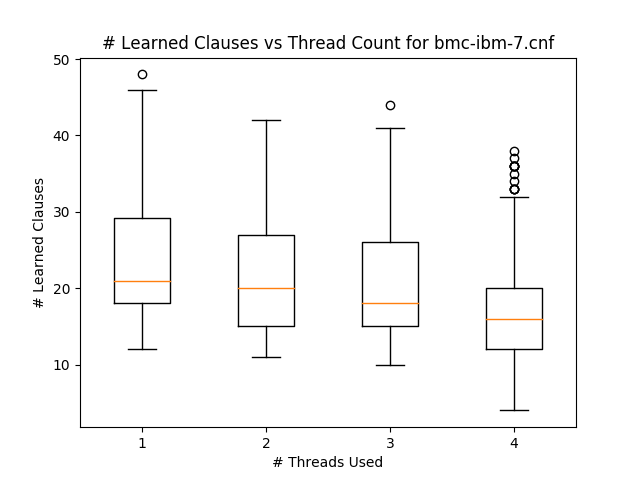
\includegraphics[width=0.25\textwidth]{figures/bmc-ibm-7lnt.png}
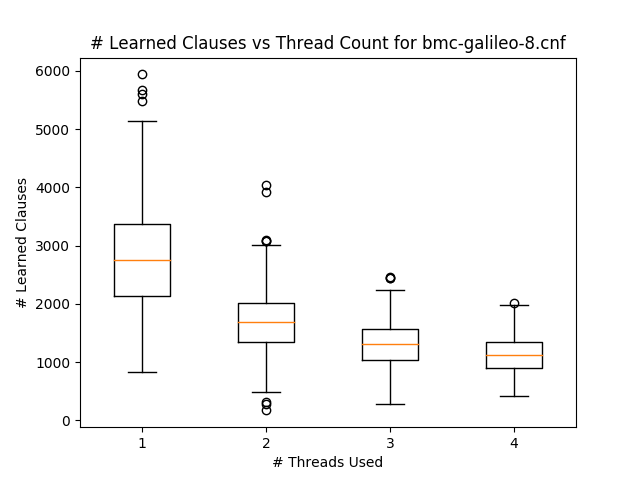
\includegraphics[width=0.25\textwidth]{figures/bmc-galileo-8lnt.png}
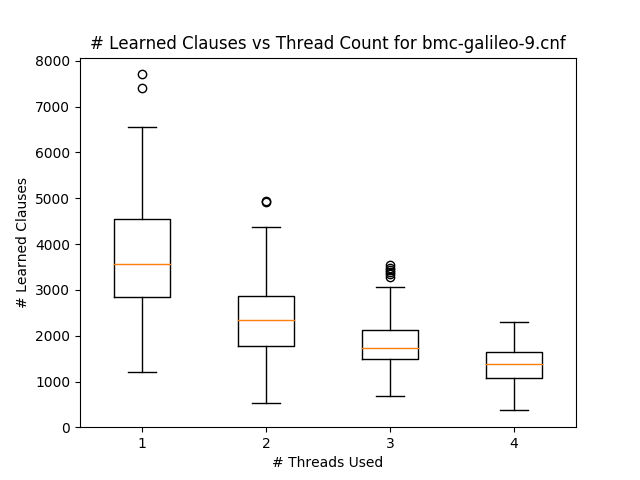
\includegraphics[width=0.25\textwidth]{figures/bmc-galileo-9lnt.png}
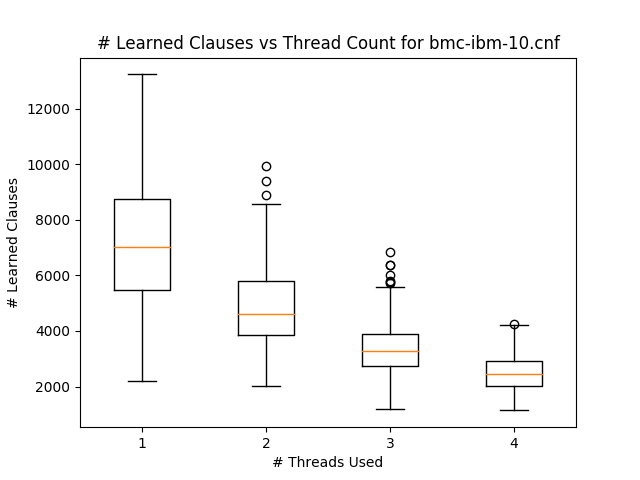
\includegraphics[width=0.25\textwidth]{figures/bmc-ibm-10lnt.png}
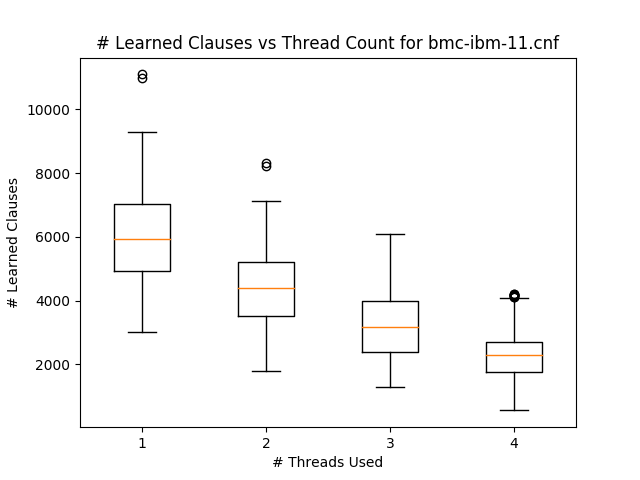
\includegraphics[width=0.25\textwidth]{figures/bmc-ibm-11lnt.png}
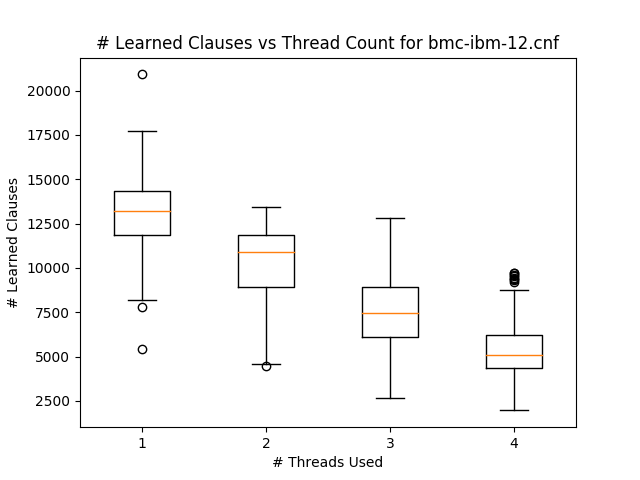
\includegraphics[width=0.25\textwidth]{figures/bmc-ibm-12lnt.png}
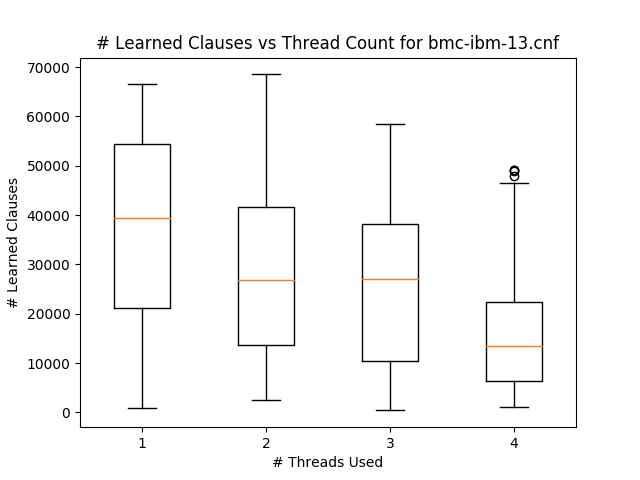
\includegraphics[width=0.25\textwidth]{figures/bmc-ibm-13lnt.png}

Interestingly, as the number of threads increases, the amount of conflicts that are performed
goes down. That is, each solver is importing useful clauses which would otherwise need to have
been computed in the future. Thus, per each thread, the number of clauses learned is
significantly lower in almost all cases the more threads there are, which is a strong indication
that work is being split well amongst different solvers.

\bibliographystyle{unsrt}
\nocite{*}
\bibliography{refs.bib}

\end{document}
